\documentclass[11pt]{article}
\usepackage[margin=1in]{geometry}
\usepackage{booktabs}
\usepackage{hyperref}
\usepackage{xcolor}
\usepackage{tikz}
\usepackage{enumitem}
\usetikzlibrary{arrows.meta,positioning,shapes.geometric}

\title{Agent Coding and Token Economy: A Survey of TUI Agents, IDE Agents, Work Agents, and Context Optimization Infrastructure}
\author{Agent Roadmap Research Draft}
\date{Draft v0.3 --- June 2026}

\begin{document}
\maketitle

\begin{abstract}
AI coding agents have moved from inline code completion toward terminal-native developer shells, editor-resident collaborators, and autonomous work agents capable of planning, editing, testing, and submitting software artifacts. At the same time, long-running agent loops expose a second infrastructure problem: token economy. Agent systems must decide what context to load, what to compress, what to remember, and what to verify. This survey proposes a taxonomy of agent coding systems and context optimization infrastructure. We distinguish TUI agents, IDE agents, work agents, agent frameworks, memory layers, context middleware, agent skills, and parallel-agent infrastructure. We also introduce MiWork as a case study for a model-specific work agent combining Mimo-adapted runtime, token compression, and workflow execution. This document is a research scaffold rather than a submission-ready survey.
\end{abstract}

\section{Introduction}
Large language models (LLMs) have transformed software engineering tools from autocomplete systems into agentic systems that can inspect repositories, call tools, run tests, edit files, and coordinate multi-step plans. The visible product surface now includes terminal coding agents such as Claude Code and Aider, IDE agents such as Cursor, Trae, Qoder and Cline, and work agents such as Devin, Kimi Work, Jules and Qoder Work. These tools differ not only in user interface but also in context strategy, memory design, model targeting, and degree of autonomy.

A central theme of this survey is that agent performance is increasingly constrained by context and token economics. The question is no longer only which model can write better code; it is also which runtime can deliver the right context at the right time, avoid redundant tool outputs, preserve useful memory, coordinate parallel workers, and verify generated claims.

\section{Background}
A coding agent can be described as an LLM-driven process that observes a software environment, reasons over user goals, acts through tools, and produces reviewable artifacts. In practice, agents combine prompts, file-system tools, shell execution, Git integration, repository indexing, and external services through protocols such as MCP \cite{mcp}.

\section{Formal Definitions}
\textbf{Definition 1: Coding Agent.} A coding agent is a software system that maps a natural-language software task and an environment state to a sequence of tool-mediated actions and reviewable software artifacts.

\textbf{Definition 2: Work Agent.} A work agent is a coding agent with persistent task state, autonomous planning, execution monitoring, artifact delivery, and review workflows.

\textbf{Definition 3: Token Economy Layer.} A token economy layer is any component that reduces, routes, caches, filters, summarizes, verifies, or externalizes context so that a model receives higher-signal input under a token budget.

\textbf{Definition 4: Agent Skill.} An agent skill is a reusable instruction, rule, script, or workflow artifact that changes agent behavior without replacing the underlying runtime.

\section{Taxonomy of Coding Agents}
Table~\ref{tab:taxonomy} summarizes the core categories used in Agent Roadmap.

\begin{table}[h]
\centering
\small
\begin{tabular}{llll}
\toprule
Category & Interface & Unit of Work & Examples \\
\midrule
TUI Agent & Terminal & Diff / command loop & Claude Code, Aider \\
IDE Agent & Editor & File / feature & Cursor, Trae, Qoder \\
Work Agent & Web / Desktop & Task / PR & Devin, Jules, Kimi Work \\
Framework & Library & Runtime graph & LangGraph, AutoGen \\
Middleware & Proxy / MCP & Context route & Entroly, LeanCTX \\
Memory Layer & CLI / MCP & Recall & ICM, Mem0, Letta \\
Skill & Rule / prompt & Behavior & SKILL.md, Cursor Rules \\
Parallel Infra & Git / AST & Coordination & Grit, worktrees \\
\bottomrule
\end{tabular}
\caption{A compact taxonomy of agent coding systems.}
\label{tab:taxonomy}
\end{table}

\section{TUI Agents}
Terminal agents expose AI coding as a developer shell. They are effective because they sit close to Git, shells, test runners, package managers, and repository files. Claude Code popularized a terminal-native agent workflow with tool approvals, skills and subagents \cite{anthropic_claude_code}. Aider provides a mature open-source pair-programming workflow with explicit file context and Git commits \cite{aider}. OpenCode and model-specific agents such as Qwen Code or DeepSeek-oriented TUIs show that the terminal surface is becoming a model runtime rather than a mere chat interface.

\section{IDE Agents}
IDE agents integrate AI into the editor surface. Cursor, Trae, Qoder, Zed, Cline and Roo Code differ in autonomy and model strategy. The IDE surface provides code navigation, inline diffs, diagnostics, and human review loops. However, the market is crowded and differentiation increasingly depends on context engineering, project memory, workflow automation and ecosystem integration \cite{cline,qoder,trae}.

\section{Work Agents}
Work agents operate on larger units: tickets, feature requests, refactors, bug fixes, research tasks or pull requests. They typically use a planner-worker-reviewer loop. Devin, Google Jules, GitHub Copilot Coding Agent, Kimi Work and Qoder Work suggest a transition from \emph{assistant} to \emph{AI engineering unit} \cite{devin,kimi_work,github_copilot,jules}. The work-agent layer is the most relevant comparison point for MiWork.

\section{Token Economy and Context Optimization}
Token economy includes command-output filtering, context compression, retrieval, memory, cache alignment, and hallucination verification. Tools such as rtk and Lowfat reduce shell-output tokens \cite{rtk,lowfat}. Entroly and LeanCTX operate as context control planes \cite{entroly}. CodeAgents proposes codified multi-agent reasoning for token-efficient planning \cite{codeagents2025}, while SupervisorAgent explores runtime supervision to reduce wasted reasoning \cite{supervisoragent2026}.

\begin{figure}[h]
\centering
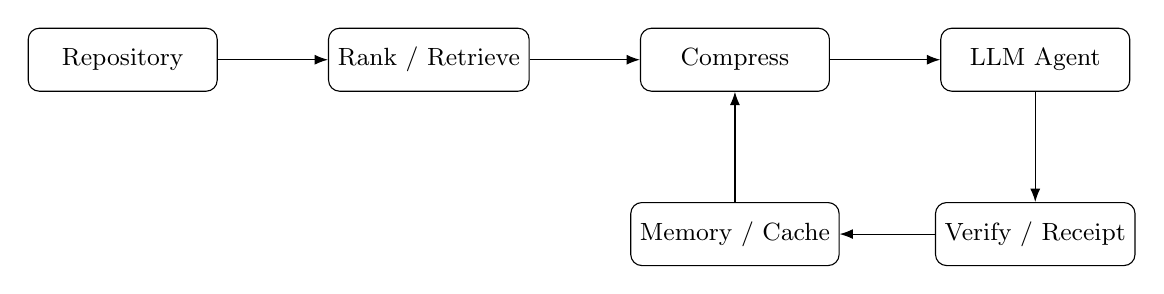
\begin{tikzpicture}[node distance=1.4cm, every node/.style={font=\small}, box/.style={draw, rounded corners, align=center, minimum width=2.4cm, minimum height=.8cm}]
\node[box] (repo) {Repository};
\node[box, right=of repo] (rank) {Rank / Retrieve};
\node[box, right=of rank] (compress) {Compress};
\node[box, right=of compress] (model) {LLM Agent};
\node[box, below=of compress] (memory) {Memory / Cache};
\node[box, below=of model] (verify) {Verify / Receipt};
\draw[-{Latex}] (repo) -- (rank);
\draw[-{Latex}] (rank) -- (compress);
\draw[-{Latex}] (compress) -- (model);
\draw[-{Latex}] (memory) -- (compress);
\draw[-{Latex}] (model) -- (verify);
\draw[-{Latex}] (verify) -- (memory);
\end{tikzpicture}
\caption{A generic token optimization pipeline for coding agents.}
\label{fig:pipeline}
\end{figure}

\section{Agent Memory and Multi-Agent Coordination}
Memory systems such as ICM, Mem0, Letta, Claude Code memory setups and MCP memory servers externalize recurring project facts \cite{icm,mem0,letta}. Multi-agent coordination systems such as Grit reduce wasted work through worktree isolation and function-level locks \cite{grit}. These components are essential when a work agent scales from a single coding loop to multiple parallel workers.

\section{Benchmark Taxonomy}
A useful benchmark suite for agent systems should include task success, token cost, latency, reviewability, context quality, coordination and UX. Table~\ref{tab:benchmarks} summarizes representative benchmarks.

\begin{table}[h]
\centering
\small
\begin{tabular}{llll}
\toprule
Benchmark & Domain & Signal & Limitation \\
\midrule
HumanEval & Code generation & Pass@k & Short functions \\
SWE-bench & GitHub issues & Patch success & Issue-style tasks \\
GAIA & General agents & Tool reasoning & Not SWE-specific \\
WebArena & Web agents & Browser tasks & Web-only \\
Web-Bench & Web projects & Sequential features & New benchmark \\
SWE-Skills-Bench & SWE skills & Skill utility & Narrow intervention \\
\bottomrule
\end{tabular}
\caption{Benchmark taxonomy for coding agents and agent infrastructure.}
\label{tab:benchmarks}
\end{table}

Existing benchmarks such as SWE-bench are important but insufficient for token economy; future benchmarks should report cost, context selection quality and reviewability alongside correctness \cite{swebench,webbench,swe_skills_bench,webarena,gaia,humaneval}.

\section{UI / UX Considerations}
Agent UX is not cosmetic. It defines user trust, task handoff, approval boundaries and error recovery. A research atlas should expose taxonomy, evidence and comparison views. A work agent should show plans, progress, diffs, tests, cost and residual risks. For MiWork, UI should communicate not just what the agent did but also which context was used and why.

\section{MiWork Case Study}
We define MiWork as:
\begin{quote}
MiWork = Mimo-specific Agent Runtime + Token Compression + Work Agent Workflow.
\end{quote}
The opportunity is not to clone Cursor or Trae. Instead, MiWork should target model-specific optimization for Mimo and adjacent Chinese model ecosystems such as DeepSeek, Qwen and Kimi. A minimal roadmap is: research atlas, Mimo CLI/TUI, context compression layer, desktop/web work agent, multi-agent worktree execution, and enterprise workflow automation.

\begin{figure}[h]
\centering
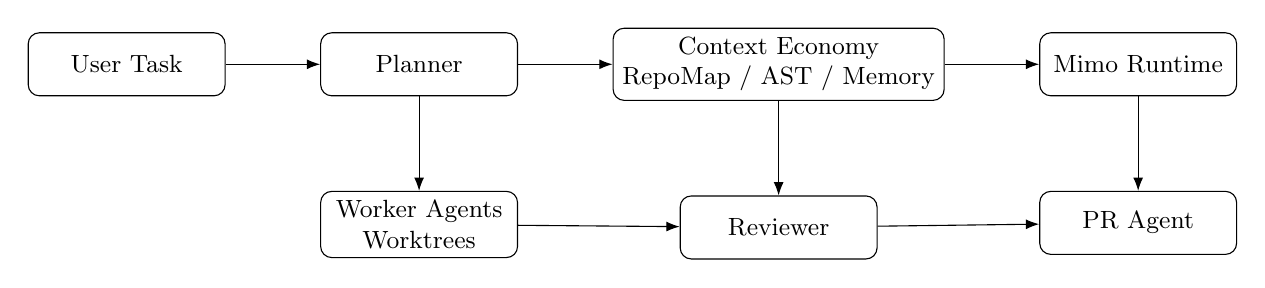
\begin{tikzpicture}[node distance=1.2cm, every node/.style={font=\small}, box/.style={draw, rounded corners, align=center, minimum width=2.5cm, minimum height=.8cm}]
\node[box] (task) {User Task};
\node[box, right=of task] (planner) {Planner};
\node[box, right=of planner] (context) {Context Economy\\RepoMap / AST / Memory};
\node[box, right=of context] (runtime) {Mimo Runtime};
\node[box, below=of planner] (workers) {Worker Agents\\Worktrees};
\node[box, below=of context] (review) {Reviewer};
\node[box, below=of runtime] (pr) {PR Agent};
\draw[-{Latex}] (task) -- (planner);
\draw[-{Latex}] (planner) -- (context);
\draw[-{Latex}] (context) -- (runtime);
\draw[-{Latex}] (planner) -- (workers);
\draw[-{Latex}] (context) -- (review);
\draw[-{Latex}] (runtime) -- (pr);
\draw[-{Latex}] (workers) -- (review);
\draw[-{Latex}] (review) -- (pr);
\end{tikzpicture}
\caption{MiWork architecture sketch.}
\label{fig:miwork}
\end{figure}

\section{Related Work}
Related systems span five areas. First, coding assistants and agents include Claude Code, Codex, Copilot, Aider, Cline and Qoder \cite{anthropic_claude_code,aider,cline,qoder,github_copilot}. Second, work agents such as Devin, Jules and Kimi Work target asynchronous issue-to-PR execution \cite{devin,jules,kimi_work}. Third, orchestration frameworks such as LangGraph, AutoGen, CrewAI, smolagents, MetaGPT and AgentScope provide abstractions for stateful or multi-agent workflows \cite{langgraph,autogen,crewai,smolagents,metagpt,agentscope}. Fourth, token economy middleware such as rtk, Entroly, Lowfat and LiteLLM address cost, context routing and provider abstraction \cite{rtk,entroly,lowfat,litellm}. Fifth, memory systems and protocols such as ICM, Mem0, Letta and MCP externalize project memory and tool access \cite{icm,mem0,letta,mcp}.

\section{Open Problems}
\begin{itemize}[leftmargin=*]
  \item \textbf{Context pollution}: more context can reduce reasoning quality.
  \item \textbf{Verification}: agents need cheap, local checks for unsupported claims.
  \item \textbf{Security}: tool access must respect least privilege.
  \item \textbf{Cost control}: token usage must be visible to users and teams.
  \item \textbf{Benchmark design}: success rates should be paired with token and review metrics.
  \item \textbf{Human trust}: users need transparent plans, diffs, tests and rollback.
\end{itemize}

\section{Conclusion}
Agent coding is evolving into a layered stack: user interface, agent runtime, context economy, memory, verification and workflow coordination. MiWork can compete by focusing on model-specific adaptation, token compression, and end-to-end workflow delivery rather than another generic IDE. This draft provides the first scaffold for a deeper survey and product roadmap.

\bibliographystyle{plain}
\bibliography{references}

\end{document}
